%!TEX root = DMmidterm.tex


\section{Project implementation}
\label{sec:projectImplementation}
In this section we present our implementation of the project in three phases. Dataset, Algorithm training, and Validation and analysis. 

\subsection{Phase I: Dataset}
\label{sec:dataset}
To add ...

%Pre-Defined Attributes


\subsection{Phase II: Algorithm Training}
\label{sec:training}

Pig To add ...
\begin{figure}[h!]
	\begin{center}
		\includegraphics[width=1\columnwidth]{/Users/MariaFerman/Desktop/DC_FinalProject/images/PigDiagram}
		\caption{Pig Diagram}
		\label{fig:dataDiagr}
	\end{center}
	\vspace{-10pt}
\end{figure}

Hive To add ...
\begin{figure}[h!]
	\begin{center}
		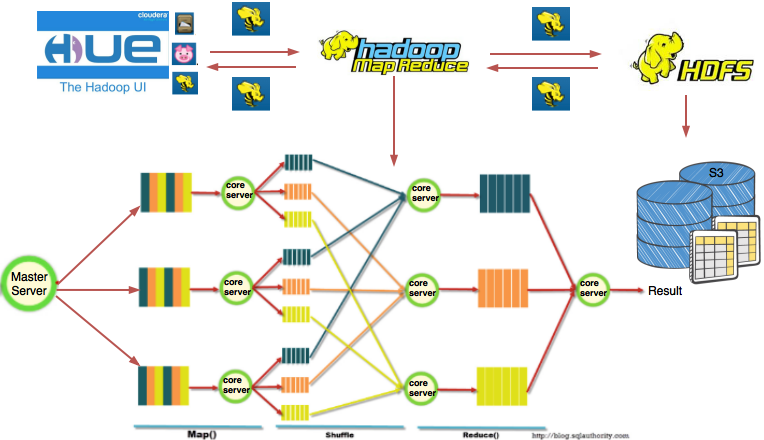
\includegraphics[width=1\columnwidth]{/Users/MariaFerman/Desktop/DC_FinalProject/images/HiveDiagram-2}
		\caption{Hive Diagram}
		\label{fig:dataDiagr}
	\end{center}
	\vspace{-10pt}
\end{figure}
(change subtitle to script?) 
